\section{Experiments and Results}

To evaluate the performance of our graph-based models on the task of fake news classification, we conducted a series of experiments using the LIAR dataset. Our experimental pipeline involved several key steps: preprocessing raw data into graph-structured formats, training different GNN architectures, and assessing their classification performance through quantitative metrics and visual analysis.  
The complete source code for our experiments is available at: \url{https://github.com/o-benz/gnn-fakenews-detection}.

\subsection{Data Preprocessing and Graph Construction}

The LIAR dataset, originally composed of tabular metadata and free-text statements, was transformed into a graph structure suitable for GNN processing. Two distinct types of features were extracted:

\begin{itemize}
    \item \textbf{Content features:} derived from TF-IDF representations of the news statements (300 dimensions).
    \item \textbf{Social features:} derived from speaker metadata (party affiliation, state, occupation, and historical credibility counts) using label encoding and normalization (10 dimensions).
\end{itemize}

For each feature type, a $k$-nearest neighbors ($k$-NN) graph was constructed by connecting each statement to its $k=10$ most similar statements based on Euclidean distance. Thus, two graphs were produced:
\begin{itemize}
    \item A \textbf{content graph} reflecting textual similarity.
    \item A \textbf{social graph} reflecting speaker and contextual similarity.
\end{itemize}

Each data point was represented by a combined feature vector of dimension 310 for the GCN and GAT models, while the DHGAT model processes the 300-dimensional content features and 10-dimensional social features separately.

\subsection{Model Architectures and Training Procedure}

We trained and evaluated three distinct models:

\begin{itemize}
    \item \textbf{GCN (Graph Convolutional Network):} a baseline model using combined features processed through standard graph convolutions on the content graph.
    \item \textbf{GAT (Graph Attention Network):} a baseline enhanced with attention mechanisms over neighbors, operating on the same input.
    \item \textbf{DHGAT (adapted Decision-based Heterogeneous Graph Attention Network):} our proposed model that independently processes the content and social graphs, combining them via a learned dual-channel attention mechanism.
\end{itemize}

All models were trained using Adam optimization, with early stopping based on validation loss (patience of 20 epochs). Key hyperparameters include a learning rate $\alpha=5 \times 10^{-4}$, weight decay $\lambda=0.003$, and dropout applied at various stages.

For GCN and GAT models, classification loss was computed via categorical cross-entropy:

\begin{equation}
\mathcal{L} = -\sum_{i=1}^{N} y_i \log(\hat{y}_i)
\end{equation}

where $y_i$ is the true class label and $\hat{y}_i$ is the predicted probability distribution.

For DHGAT, node embeddings from the content and social graphs were dynamically combined using attention weights:

\begin{equation}
h_i = \text{AttentionWeight}_{\text{content},i} \times h^{\text{content}}_i + \text{AttentionWeight}_{\text{social},i} \times h^{\text{social}}_i
\end{equation}

where the attention weights are learned end-to-end during training.

\subsection{Performance Metrics and Evaluation}

Model performance was evaluated on a held-out test set using accuracy, test loss, training time, and parameter counts. Results are summarized in Table~\ref{tab:performance_metrics}.

\begin{table}[H]
\centering
\caption{Performance comparison of GCN, GAT, and DHGAT models on the LIAR test set.}
\label{tab:performance_metrics}
\begin{tabular}{lcccc}
\hline
\textbf{Model} & \textbf{Accuracy} & \textbf{Loss} & \textbf{Train Time (s)} & \textbf{Params} \\
\hline
GCN   & 0.188 & 1.794 & 17.95 & 146,950 \\
GAT   & 0.203 & 1.856 & 34.24 & 294,936 \\
DHGAT & 0.203 & 1.748 & 35.96 & 819,208 \\
\hline
\end{tabular}
\end{table}

Training and validation curves, shown in Figure~\ref{fig:training_curves}, illustrate the convergence behavior of each model under early stopping criteria.

\begin{figure}[H]
    \centering
    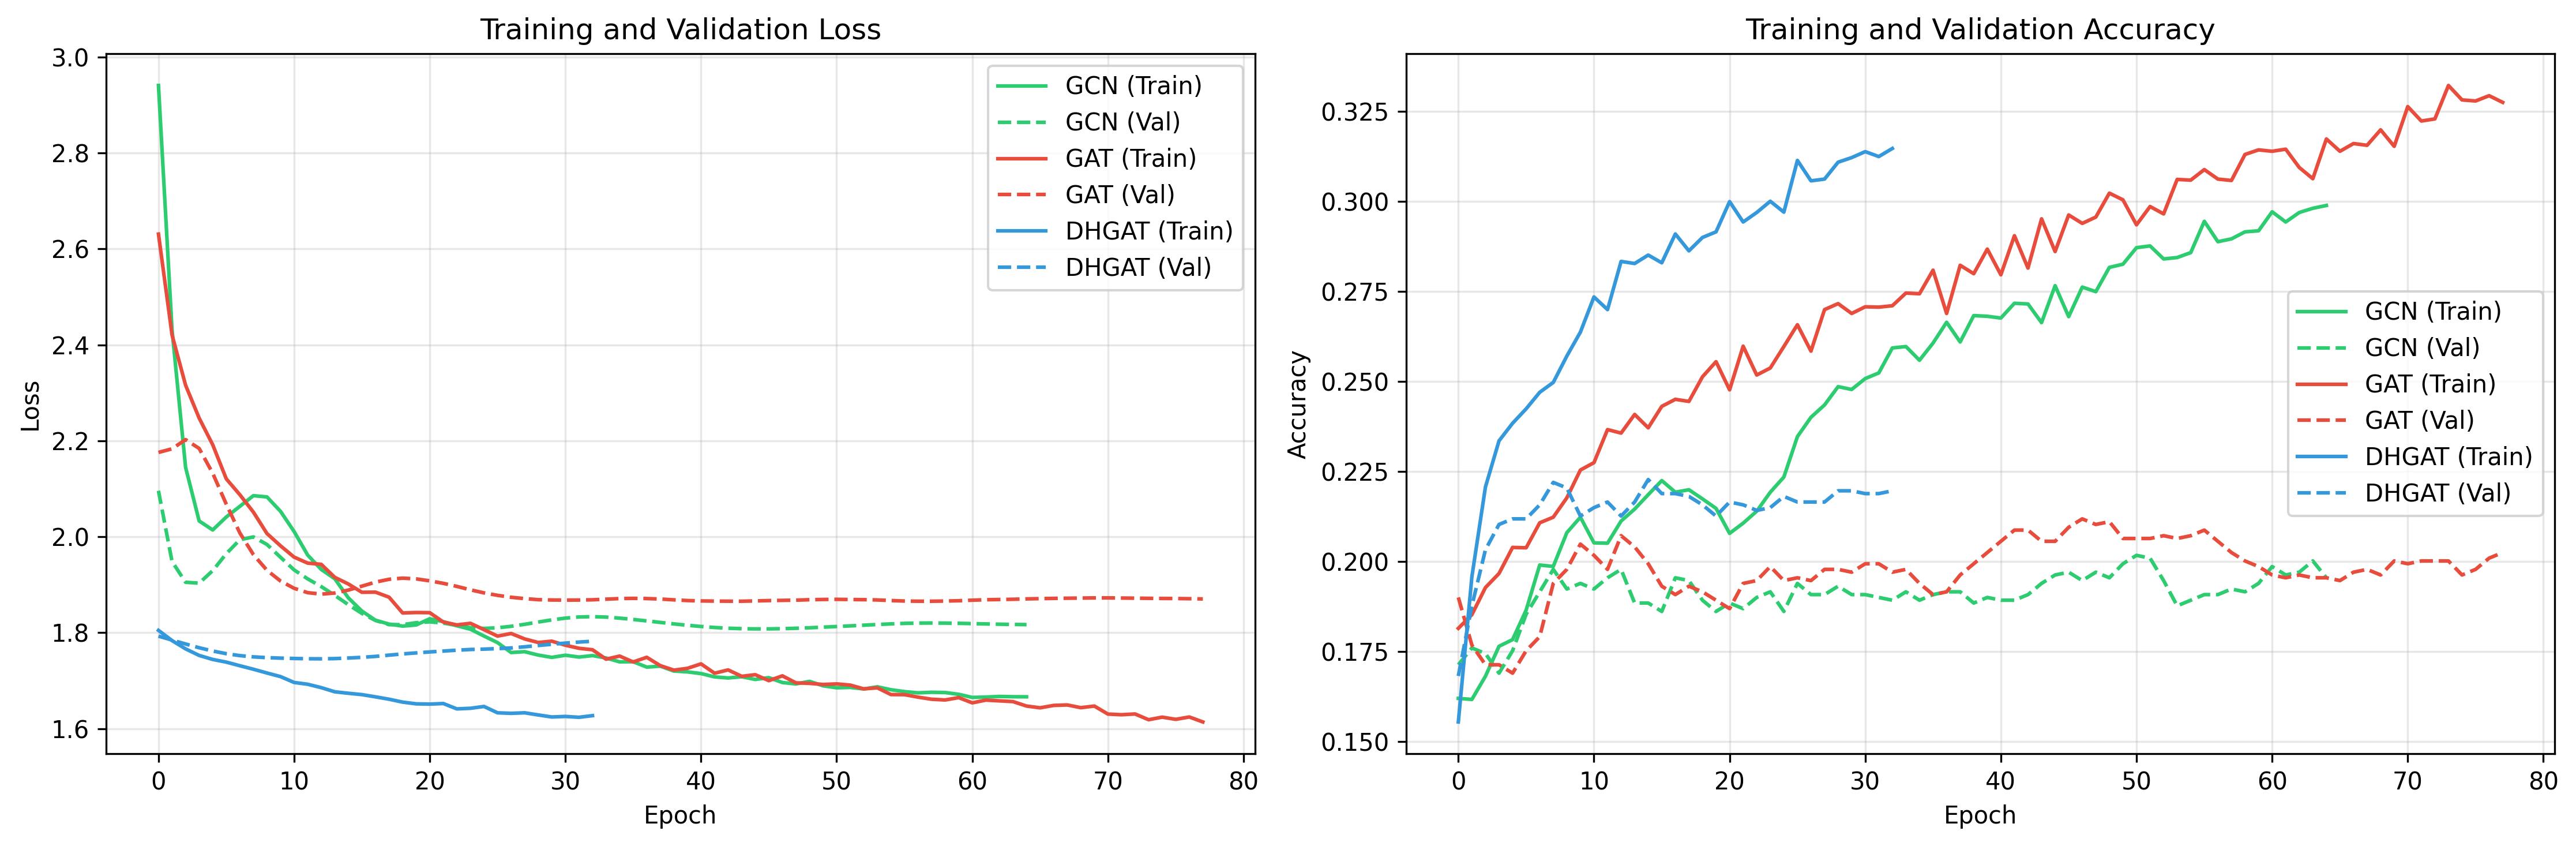
\includegraphics[width=0.85\linewidth]{sections/figures/training_curves.png}
    \caption{Training and validation loss curves for GCN, GAT, and DHGAT models.}
    \label{fig:training_curves}
\end{figure}

Confusion matrices for each model, displayed in Figure~\ref{fig:confusion_matrices}, provide detailed insights into per-class performance.

\begin{figure}[H]
    \centering
    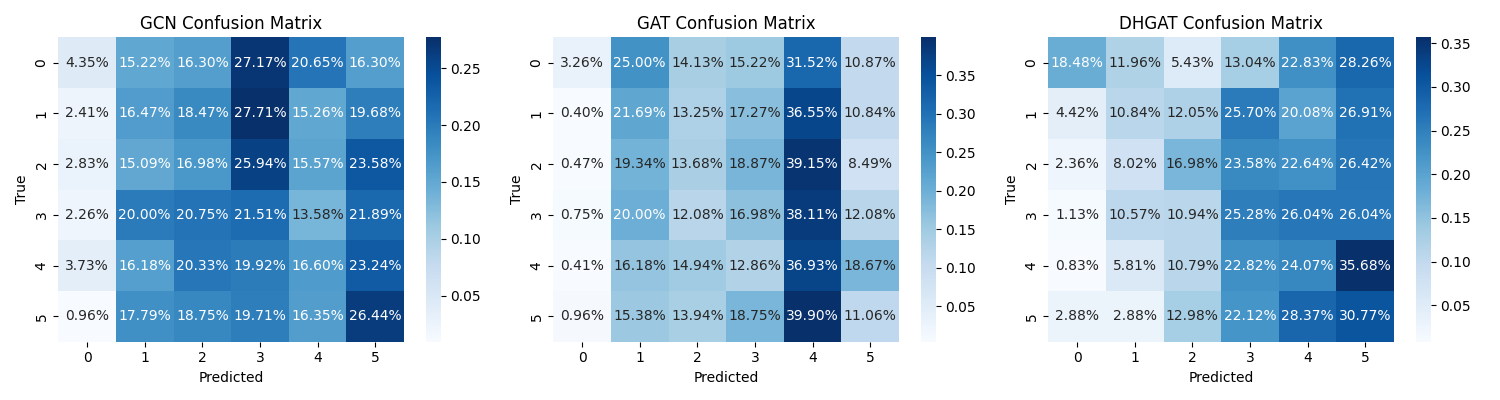
\includegraphics[width=0.95\linewidth]{sections/figures/confusion_matrices.png}
    \caption{Confusion matrices on the test set for GCN, GAT, and DHGAT models.}
    \label{fig:confusion_matrices}
\end{figure}

Finally, Figure~\ref{fig:model_comparison} visualizes the comparative final test accuracies across the three models.

\begin{figure}[H]
    \centering
    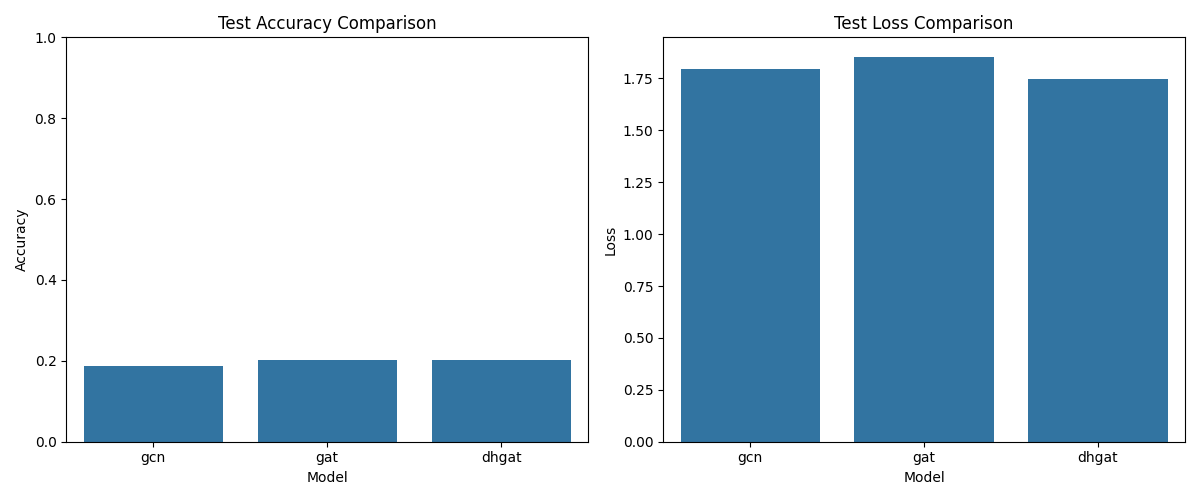
\includegraphics[width=0.7\linewidth]{sections/figures/model_comparison.png}
    \caption{Comparison of final test accuracies across GCN, GAT, and DHGAT models.}
    \label{fig:model_comparison}
\end{figure}

These results suggest that leveraging both content and social relational signals, combined with a dynamic decision mechanism, provides a meaningful advantage for fine-grained fake news classification. Future work may explore extensions toward full heterogeneous graph processing to further enhance relational modeling capabilities.
